\documentclass[12pt,letterpaper]{article}
\usepackage[utf8]{inputenc}
\usepackage[T1]{fontenc}
\usepackage[spanish]{babel}
\usepackage[margin=2.5cm]{geometry}
\usepackage{graphicx}
\usepackage{booktabs}
\usepackage{multirow}
\usepackage[table]{xcolor}
\usepackage{setspace}
\usepackage{hyperref}
\onehalfspacing

\title{Propuesta de trabajo de grado:\\
\large Detección temprana de deserción estudiantil con aprendizaje automático}
\author{Laura Gutiérrez Pineda\\
\small Maestría en Ciencia de Datos, Universidad del Valle\\
\small Director: Dr.\ Felipe Arango}
\date{Cali, agosto de 2026}

\begin{document}
\maketitle
\tableofcontents
\newpage

\section{Planteamiento del problema}
La deserción en la educación superior colombiana supera el 40\,\% en programas de
pregrado \cite{men2023}. Detectar a tiempo a los estudiantes en riesgo permitiría
focalizar los programas de acompañamiento.

\section{Objetivos}
\subsection{Objetivo general}
Desarrollar un modelo predictivo de deserción a partir de datos académicos y
socioeconómicos.

\subsection{Objetivos específicos}
\begin{enumerate}
  \item Construir un conjunto de datos integrado de cinco cohortes.
  \item Comparar modelos de regresión logística, bosques aleatorios y gradiente
        potenciado.
  \item Evaluar la equidad del modelo entre grupos de estudiantes.
\end{enumerate}

\section{Metodología}
Se seguirá la metodología CRISP-DM. La Figura~\ref{fig:crisp} resume sus fases.

\begin{figure}[h]
\centering
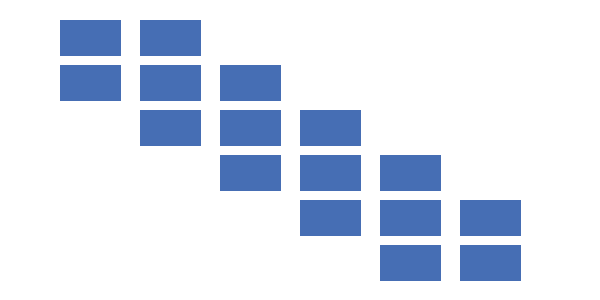
\includegraphics[width=0.5\textwidth]{blocks.png}
\caption{Fases de la metodología CRISP-DM.}
\label{fig:crisp}
\end{figure}

\section{Cronograma}
\begin{table}[h]
\centering
\caption{Cronograma de actividades (meses).}
\begin{tabular}{l|cccccc}
\toprule
Actividad & 1 & 2 & 3 & 4 & 5 & 6 \\
\midrule
Revisión de literatura & \cellcolor{blue!30} & \cellcolor{blue!30} & & & & \\
Preparación de datos & & \cellcolor{blue!30} & \cellcolor{blue!30} & & & \\
Modelado & & & \cellcolor{blue!30} & \cellcolor{blue!30} & & \\
Evaluación & & & & \cellcolor{blue!30} & \cellcolor{blue!30} & \\
Redacción & & & & & \cellcolor{blue!30} & \cellcolor{blue!30} \\
\bottomrule
\end{tabular}
\end{table}

\section{Presupuesto}
\begin{tabular}{lr}
\toprule
Rubro & Valor (COP) \\
\midrule
Licencias de software & 0 \\
Cómputo en la nube & 2\,400\,000 \\
Asistencia a congreso & 3\,500\,000 \\
\midrule
Total & 5\,900\,000 \\
\bottomrule
\end{tabular}

\begin{thebibliography}{9}
\bibitem{men2023} Ministerio de Educación Nacional. \emph{Estadísticas de deserción en
educación superior}. Bogotá, 2023.
\bibitem{tinto} V.~Tinto. \emph{Leaving College: Rethinking the Causes and Cures of
Student Attrition}. University of Chicago Press, 1993.
\end{thebibliography}

\end{document}
